\documentclass{article}
\usepackage[utf8]{inputenc}
\usepackage[swedish]{babel}
\usepackage{authblk}
\usepackage{biblatex}
\addbibresource{sources.bib}
\usepackage{graphicx}

\title{ProjektRapport 14}
\author{Alamin Alreda \and Sebastian Danckwardt \and Isac Holm \and Zaid Haj Ibrahim   \and Edvin Svahn}
\date{September 2022}

\begin{document}

\maketitle
 
\section{Introduction}
\subsection{Syfte}
Varför?
\\
Bara under 2021 har 72 884 fall av inbrottsstöld anmälts\cite{BRa}. 
Cirka 20\% svarar att de inte har ett hemlarm för att det helt enkelt är för dyrt\cite{MoFor}.
Genom att skapa ett system med ett billigt md407-kort kan man sänka kostnaderna för denna produkt och bekämpa brott i alla områden i Sverige. 
Projektet syftar till att skapa ett lättanvändligt och billigt larmsystem för att skydda mot stöld. 
Detta då endast 29\% av Sveriges befolkning idag använder ett larmsystem\cite{SSF}.
\subsection{Mål}
Vad?
\\
Målet med projektet är att konstruera ett larm/lås-system med två olika larmenheter: 
den ena ska kunna upptäcka i fall en dörr står öppen och den andra ska detektera rörelse och vibrationer. 
En central styrenhet ska utgöra den del av larmsystemet som har i uppgift att kommunicera med de fristående larmenheterna. 
Detta ska möjliggöra centraliserad kontroll och kalibrering av flera periferienheter i ett större larmsystem. 
Ytterligare en periferienhet ska simulera ett defekt larm i syfte för testning.
\\\\
När den centrala styrenheten startar ska en förfrågan skickas till de anslutna periferienheterna därpå de svarar med dess typ och konfiguration för att sedan tilldelas ett unikt ID. De olika larmenheterna ska inledningsvis larma lokalt med en röd lysdiod, om specifika krav nås meddelas den centrala styrenheten. Dörrlarmet larmar till centralenheten efter en bestämd tid medans rörelsesensorn måste upptäcka rörelse på ett visst avstånd. Det ska även vara möjligt att låsa/låsa upp dörren samt inaktivera dörrlarmet genom att mata in en fyrsiffrig kod på en keypad.


\subsection{Arbetsmetod}
Hur har vi gått tillväga i det tekniska utvecklingsarbetet

\section{Teknisk beskrivning}
I det här kapitlet redogörs projektets tekniska bedrifter. 
I den tekniska bakgrunden beskrivs varför systemet är uppbyggt av de delar som det är.
Därefter ger Systemöversikten en övergripande förståelse för hur systemet är uppbyggt och sist men inte minst förklarar Delsystem hur delarna är uppbyggda.


\subsection{Teknisk bakgrund}
Vad är utgångspunkten för konstruktionsarbetet?

\subsection{Systemöversikt}
Hur ser det konstruerade systemet ut på en övergripande nivå?
/h



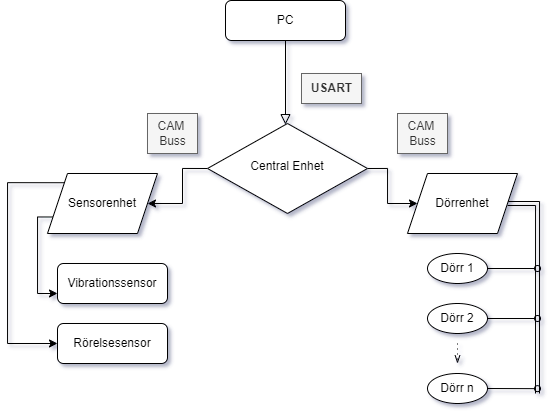
\includegraphics[scale=0.6]{Projektrapport/diagram.png}
\caption {Blockschema av larmsystemet}
\label{fig:drawing}


Systemet består i stort av tre delar - en centralenhet och två periferienheter. Utöver dessa enheterna innehåller systemet övriga delenheter som bidrar till funktionalitet av systemet i sin helhet. Ett md407-kort används som en ARM-processor för att koppla ihop olika instrument beroende på deras funktion och uppgifter (figure 1). Kommunikation mellan samtliga md-kort sker via CAN-buss, medan kommuniaktion mellan centralenheten och pc sker över USART. \\


Periferienhet 1 ska vara ansluten till en kopplingsplatta, på plattan ska det finnas lampor och en dörr-strömbrytare. Lamporna kommer lysa rött efter att dörren har varit öppen en viss tid eller grönt om inget larm har gått. Dörr-strömbrytarna kommer att simulera dörröppning eller dörrstängning. \\

Periferienhet 2 ska vara kopplad till en avståndsmätare (HC-SR04) och en vibrationssensor (SW-18010P). Avståndmätaren kommer att skicka en signal om avståndet har ändrats. På samma sätt kommer vibrationssensorn skicka en signal om den har känt av några vibrationer. \\


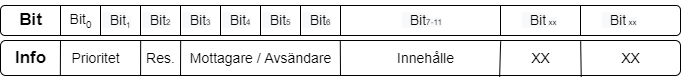
\includegraphics[scale=0.5]{Projektrapport/protokoll (1).png}

\subsection{Delsystem}
Hur ser det delar som ingår i systemet ut?

\section{Resultat}
Detta avsnitt redovisar resultatet av genomförd verifiering av systemet; dels fördelarna, dels för 
komplett system. Detta avsnitt redovisar även resultatet av det slutliga fysiska testet när hela systemet 
körs i skarpt läge. Ni ska främst redovisa resultat i form av funktionalitet, men ta också upp prestanda 
aspekter om dessa är viktiga.  
\section{Slutsatser}
\newpage
\section{Källförteckning}
\printbibliography[title=\n]

\end{document}
